\documentclass[tikz, border=10pt]{standalone}
\usepackage{tikz}
\usetikzlibrary{positioning}
\usetikzlibrary{arrows.meta}
\usetikzlibrary{shapes.geometric}
\usetikzlibrary{decorations.pathmorphing}
\usetikzlibrary{fit}
\pgfdeclarelayer{background}
\pgfsetlayers{background,main}

\begin{document}

% \begin{tikzpicture}[
%         entity/.style={draw, rounded corners, fill=blue!10, minimum width=3.2cm, minimum height=1cm, font=\small, align=center},
%         attr/.style={draw, fill=white, minimum width=2.8cm, minimum height=0.8cm, font=\footnotesize, align=left},
%         rel/.style={font=\footnotesize, midway, fill=white, inner sep=1pt},
%         node distance=1.6cm and 2.5cm
%     ]

%     % Main entities
%     \node[entity] (course) {Course};
%     \node[entity, right=of course] (instructor) {Instructor};
%     \node[entity, below=of course] (group) {Group};
%     \node[entity, right=of group] (room) {Room};

%     % Course attributes
%     \node[attr, left=of course] (course_instructors) {qualified\_instructor\_ids};
%     \node[attr, below=of course_instructors] (course_groups) {group\_ids};
%     \node[attr, below=of course_groups] (course_roomtype) {required\_room\_type};

%     % Instructor attribute
%     \node[attr, above=of instructor] (inst_courses) {qualified\_courses};

%     % Group attribute
%     \node[attr, below=of group] (group_courses) {enrolled\_courses};

%     % Room attribute
%     \node[attr, below=of room] (room_type) {room\_type};

%     % Relationships
%     \draw[<->, thick] (course) -- node[rel, above] {Many to Many} (instructor);
%     \draw[<->, thick] (course) -- node[rel, right] {Many to Many} (group);
%     \draw[->, thick] (course) -- node[rel, sloped, above] {Type Requirement} (room);
%     % Attribute connections
%     \draw[dashed] (course) -- (course_instructors);
%     \draw[dashed] (course) -- (course_groups);
%     \draw[dashed] (course) -- node[rel, sloped, above] {Many to Many}(course_roomtype);

%     \draw[dashed] (instructor) -- (inst_courses);
%     \draw[dashed] (group) -- (group_courses);
%     \draw[dashed] (room) -- (room_type);

% \end{tikzpicture}




% \begin{figure}[h!]
%     \centering
%     \begin{tikzpicture}[
%             node distance=1.6cm and 1.8cm,
%             every node/.style={draw, minimum width=2.8cm, minimum height=1cm, align=center},
%             arrow/.style={->, >=Latex},
%             label/.style={font=\small}
%         ]

%         % Nodes
%         \node (latent) {Latent Space};
%         \node[right=of latent] (generator) {Generator};
%         \node[right=of generator] (genimg) {Generator Image};

%         \node[below=of latent] (dataset) {Dataset};
%         \node[right=of dataset] (realimg) {Real Image};

%         \node[below=of genimg] (discriminator) {Discriminator};
%         \node[right=of discriminator] (output) {Real or Fake};

%         % Arrows (forward)
%         \draw[arrow] (latent) -- (generator);
%         \draw[arrow] (generator) -- (genimg);
%         \draw[arrow] (genimg) -- (discriminator);
%         \draw[arrow] (dataset) -- (realimg);
%         \draw[arrow] (realimg) -- (discriminator);
%         \draw[arrow] (discriminator) -- (output);

%         % Feedback loops
%         \node[above=1.2cm of generator] (bpgen) {Back Propagation: Maximize Error};
%         \node[below=1.4cm of discriminator] (bpdisc) {Back Propagation: Minimize Error};

%         \draw[arrow] (output.north) to[out=90,in=0] (bpgen.east);
%         \draw[arrow] (bpgen.west) to[out=180,in=90] (generator.north);

%         \draw[arrow] (output.south) to[out=-90,in=0] (bpdisc.east);
%         \draw[arrow] (bpdisc.west) to[out=180,in=-90] (discriminator.south);

%     \end{tikzpicture}
%     \caption{GAN System Architecture with Forward and Backward Pass}
% \end{figure}
\begin{figure}[!htbp]
    \centering
    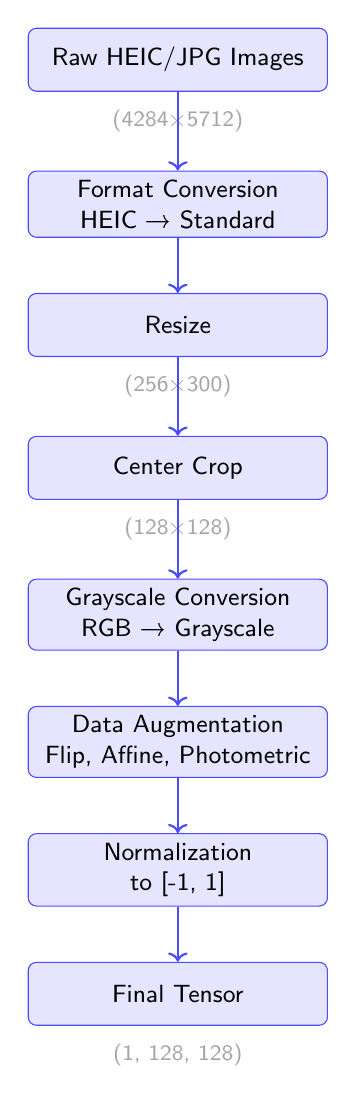
\begin{tikzpicture}[
            node distance=0.7cm,
            box/.style = {
                    rectangle,
                    draw=blue!70,
                    fill=blue!10,
                    rounded corners=3pt,
                    minimum width=3.8cm,
                    minimum height=0.8cm,
                    align=center,
                    font=\sffamily\small
                },
            arrow/.style = {->, thick, blue!70},
            dimension/.style = {font=\sffamily\footnotesize, color=gray!70}
        ]

        % Nodes with dimensions
        \node[box] (raw) {Raw HEIC/JPG Images};
        \node[dimension, below=0.1cm of raw] {(4284×5712)};

        \node[box, below=1.0cm of raw] (convert) {Format Conversion \\ HEIC → Standard};

        \node[box, below=of convert] (resize) {Resize};
        \node[dimension, below=0.1cm of resize] {(256×300)};

        \node[box, below=1.0cm of resize] (crop) {Center Crop};
        \node[dimension, below=0.1cm of crop] {(128×128)};

        \node[box, below=1.0cm of crop] (gray) {Grayscale Conversion \\ RGB → Grayscale};

        \node[box, below=of gray] (augment) {Data Augmentation \\ Flip, Affine, Photometric};

        \node[box, below=of augment] (norm) {Normalization \\ to [-1, 1]};

        \node[box, below=of norm] (tensor) {Final Tensor};
        \node[dimension, below=0.1cm of tensor] {(1, 128, 128)};

        % Arrows
        \draw[arrow] (raw) -- (convert);
        \draw[arrow] (convert) -- (resize);
        \draw[arrow] (resize) -- (crop);
        \draw[arrow] (crop) -- (gray);
        \draw[arrow] (gray) -- (augment);
        \draw[arrow] (augment) -- (norm);
        \draw[arrow] (norm) -- (tensor);

    \end{tikzpicture}
    \caption{Data Preprocessing Pipeline: Complete workflow from raw images through format conversion, geometric transformations, augmentation, and normalization to produce training-ready tensors.}
    \label{fig:preprocessing_pipeline}
\end{figure}



\begin{figure}[h!]
    \centering
    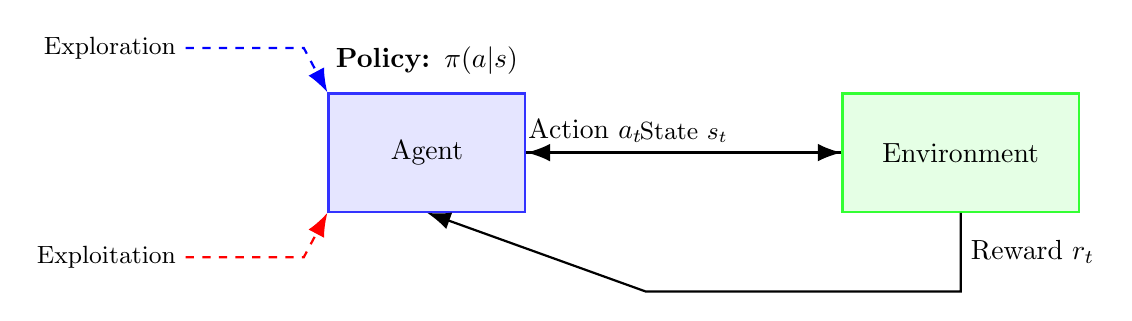
\begin{tikzpicture}[
        agent/.style={rectangle, draw=blue!80, fill=blue!10, thick, minimum width=2.5cm, minimum height=1.5cm},
        env/.style={rectangle, draw=green!80, fill=green!10, thick, minimum width=3cm, minimum height=1.5cm},
        arrow/.style={thick, -{Latex[length=3mm]}},
        label/.style={font=\small}
        ]

        % Nodes
        \node[agent] (agent) {Agent};
        \node[env, right=4cm of agent] (env) {Environment};

        % State, Action, Reward Labels
        \node[label, above left=0.3cm and 1.8cm of agent] (exploration) {Exploration};
        \node[label, below left=0.3cm and 1.8cm of agent] (exploitation) {Exploitation};

        % Arrows
        \draw[arrow] (env.west) -- node[above, label] {State $s_t$} (agent.east);
        \draw[arrow] (agent.east) -- ++(1.5, 0) node[midway, above] {Action $a_t$} -- (env.west);
        \draw[arrow] (env.south) -- ++(0,-1) node[midway, right] {Reward $r_t$} -- ++(-4, 0) -- (agent.south);

        % Dashed arrows for exploration/exploitation
        \draw[arrow, dashed, blue] (exploration.east) -- ++(1.5,0) node[midway, above] {} -- (agent.north west);
        \draw[arrow, dashed, red] (exploitation.east) -- ++(1.5,0) node[midway, below] {} -- (agent.south west);

        % Labels
        \node[above=0.1cm of agent] {\textbf{Policy: }$\pi(a|s)$};

    \end{tikzpicture}
    \caption{Reinforcement Learning Agent Interacting with Environment: Balance of Exploration and Exploitation}
\end{figure}


\begin{figure}[!htbp]
    \centering
    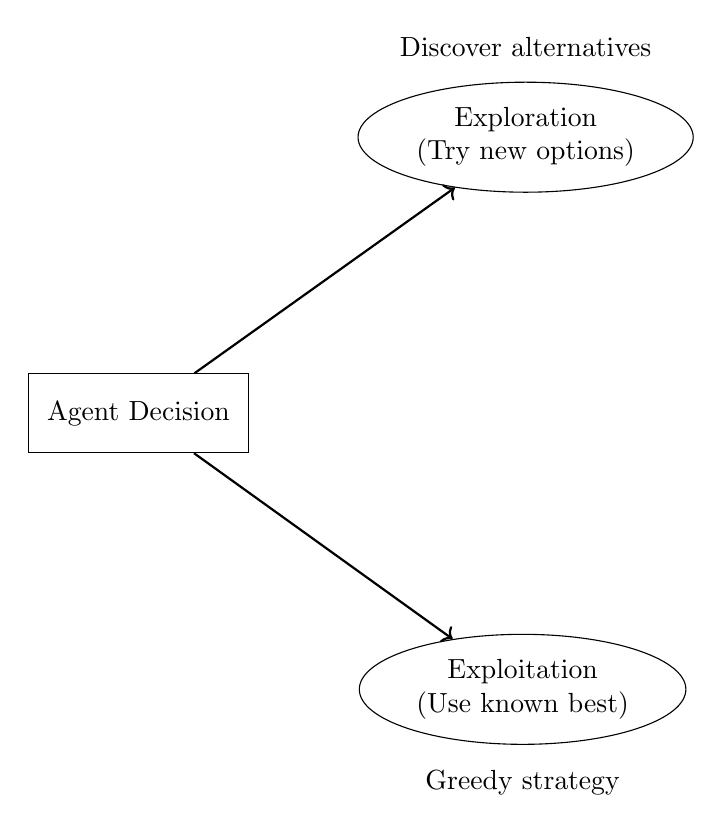
\begin{tikzpicture}[
            node distance=2.5cm and 2cm,
            decision/.style={rectangle, draw, minimum width=2.8cm, minimum height=1cm},
            path/.style={->, thick},
            option/.style={ellipse, draw, align=center, minimum width=2.5cm, minimum height=1cm}
        ]

        % Nodes
        \node[decision] (start) {Agent Decision};
        \node[option, above right=of start] (exploration) {Exploration\\(Try new options)};
        \node[option, below right=of start] (exploitation) {Exploitation\\(Use known best)};

        % Arrows
        \draw[path] (start) -- (exploration);
        \draw[path] (start) -- (exploitation);

        % Labels
        \node[below=0.2cm of exploitation] {Greedy strategy};
        \node[above=0.2cm of exploration] {Discover alternatives};

    \end{tikzpicture}
    \caption{Exploration vs. Exploitation decision in agent learning}
    \label{fig:explore_exploit}
\end{figure}


\begin{figure}[!htbp]
    \centering
    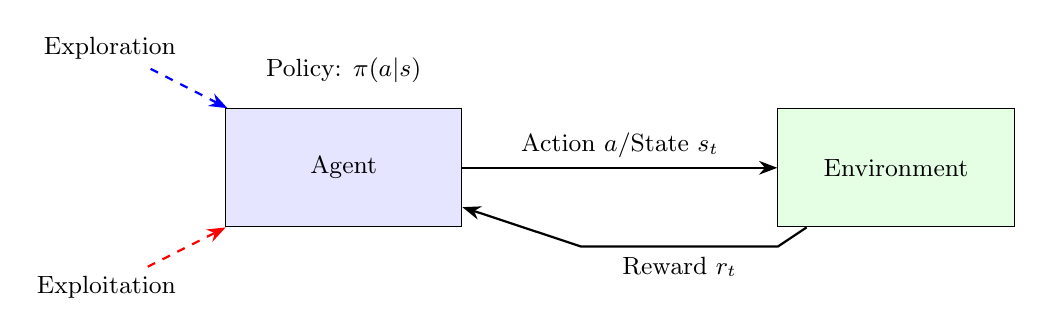
\begin{tikzpicture}[
            box/.style={draw, minimum width=3cm, minimum height=1.5cm, align=center},
            arrow/.style={thick, ->, >=Stealth},
            expl/.style={thick, dashed, ->, >=Stealth},
            font=\small
        ]

        % Nodes
        \node[box, fill=blue!10] (agent) {Agent};
        \node[box, fill=green!10, right=4cm of agent] (env) {Environment};

        % Labels
        \node[above left=0.5cm and 0.5cm of agent] (explore_label) {Exploration};
        \node[below left=0.5cm and 0.5cm of agent] (exploit_label) {Exploitation};
        \node[above=0.2cm of agent] (policy_label) {Policy: $\pi(a|s)$};

        % Arrows
        \draw[arrow] (agent) -- node[above] {Action $a$/State $s_t$} (env);
        \draw[arrow] (env) -- ++(-1.5, -1) -- node[below] {Reward $r_t$} ++(-2.5, 0) -- (agent);
        \draw[expl, blue] (explore_label) -- (agent);
        \draw[expl, red] (exploit_label) -- (agent);

    \end{tikzpicture}
    \caption{Reinforcement Learning Agent Interacting with Environment: Balance of Exploration and Exploitation}
    \label{fig:explore_exploit_rl}
\end{figure}


\begin{figure}[!htbp]
    \centering
    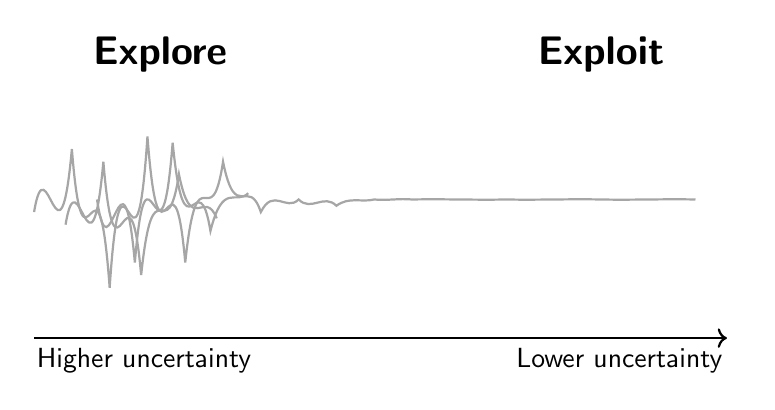
\begin{tikzpicture}[scale=0.8]

        % Draw the main curve - complex scribbling that gradually flattens (oscillating up and down)
        \draw[thick, gray!70]
        (0,2) .. controls (0.2,3.2) and (0.4,0.8) .. (0.6,3.0)
        .. controls (0.8,0.5) and (1.0,3.5) .. (1.2,0.8)
        .. controls (1.4,3.8) and (1.6,0.2) .. (1.8,3.2)
        .. controls (2.0,0.6) and (2.2,3.4) .. (2.4,1.2)
        .. controls (2.6,3.1) and (2.8,1.5) .. (3.0,2.8)
        .. controls (3.2,1.8) and (3.4,2.6) .. (3.6,2.0)
        .. controls (3.8,2.4) and (4.0,2.0) .. (4.2,2.2)
        .. controls (4.4,2.0) and (4.6,2.3) .. (4.8,2.1)
        .. controls (5.0,2.25) and (5.2,2.15) .. (5.4,2.2)
        .. controls (5.6,2.18) and (5.8,2.22) .. (6.0,2.2)
        .. controls (6.5,2.21) and (7.0,2.19) .. (7.5,2.2)
        .. controls (8.0,2.19) and (8.5,2.21) .. (9.0,2.2)
        .. controls (9.5,2.19) and (10.0,2.21) .. (10.5,2.2);

        % Add some overlapping scribbles in the exploration phase (oscillating up and down)
        \draw[thick, gray!70]
        (0.5,1.8) .. controls (0.7,3.0) and (0.9,0.6) .. (1.1,2.8)
        .. controls (1.3,0.4) and (1.5,3.2) .. (1.7,1.0)
        .. controls (1.9,2.9) and (2.1,1.3) .. (2.3,2.6)
        .. controls (2.5,1.6) and (2.7,2.4) .. (2.9,1.9);

        \draw[thick, gray!70]
        (1.0,2.2) .. controls (1.2,0.8) and (1.4,3.4) .. (1.6,1.2)
        .. controls (1.8,3.6) and (2.0,0.6) .. (2.2,3.1)
        .. controls (2.4,1.1) and (2.6,2.9) .. (2.8,1.7)
        .. controls (3.0,2.5) and (3.2,2.1) .. (3.4,2.3);

        % Horizontal axis
        \draw[->, thick] (0,0) -- (11,0) node[right] {};
        \node[below right, font=\sffamily] at (7.5, 0){Lower uncertainty};
        \node[below left, font=\sffamily] at (3.6,0) {Higher uncertainty};

        % Labels
        \node[font=\sffamily\Large\bfseries] at (2,4.5) {Explore};
        \node[font=\sffamily\Large\bfseries] at (9,4.5) {Exploit};

    \end{tikzpicture}
    \caption{Explore–Exploit Trade-off: Random exploration under high uncertainty transitioning into stable exploitation.}
    \label{fig:explore_exploit_curve}
\end{figure}

\subsection{State, Action, Reward Design}
%% bibek flowchart here
\textbf{State Space:}
The state \( s_t \) represents the current condition of the GA population. It is described using a set of summary features:
\begin{itemize}
    \item Best fitness score in generation \( t \)
    \item Average fitness of the population
    \item Diversity metric (e.g., Hamming distance between chromosomes)
    \item Operator usage history
\end{itemize}

\textbf{Action Space:}
Each action \( a_t \) is a selection or adjustment of a GA operator or its parameter. Examples include:
\begin{itemize}
    \item Selecting crossover type: one-point, two-point, uniform
    \item Selecting mutation type or intensity
    \item Adjusting mutation or crossover rate dynamically
\end{itemize}

\textbf{Reward Function:}
The agent receives feedback based on improvement in solution quality:
\begin{equation}
    r_t = f_{t} - f_{t-1}
\end{equation}
% \]
Where \( f_t \) is the best fitness at generation \( t \). The reward encourages strategies that improve the GA's convergence.

\subsection{RL Strategy for Meta-Optimization}

The RL agent interacts with GA at each generation:
\begin{itemize}
    \item Observe current state vector \( s_t \)
    \item Choose an action \( a_t \) (e.g., operator or rate)
    \item Apply the action to the GA
    \item Execute GA generation
    \item Observe new state \( s_{t+1} \) and reward \( r_t \)
    \item Update RL policy
\end{itemize}



\tikzstyle{process} = [rectangle, minimum width=2.5cm, minimum height=1cm, text centered, draw=black]
\tikzstyle{decision} = [diamond, minimum width=2cm, minimum height=1cm, text centered, draw=black]
\tikzstyle{data} = [rectangle, rounded corners, minimum width=2cm, minimum height=0.8cm, text centered, draw=black]
\tikzstyle{agent} = [rectangle, minimum width=2.5cm, minimum height=1cm, text centered, draw=black, thick]
\tikzstyle{ga} = [rectangle, minimum width=2.5cm, minimum height=1cm, text centered, draw=black, thick]
\tikzstyle{arrow} = [thick,->,>=stealth]

\begin{tikzpicture}[node distance=2.5cm]

    % RL Agent components
    \node (observe) [agent] {Observe State ($s_t$)};
    \node (action) [agent, below of=observe] {Choose Action ($a_t$)};
    \node (update) [agent, below=of action] {Update Policy ($\pi(a_t|s_t)$)};

    % State components
    \node (state) [data, right=4cm of observe] {State};

    % Action components  
    \node (action_space) [data, right=4cm of action] {Action Space};

    % GA components
    \node (apply_action) [ga, below=2.5cm of action_space] {Apply action to GA};
    \node (execute_ga) [ga, below of=apply_action] {Execute GA (New Generation)};
    \node (new_state) [ga, below of=execute_ga] {New State ($s_{t+1}$)};

    % Reward component
    \node (reward) [data, left=of new_state] {Reward ($r_t$)};

    % Arrows for main flow
    \draw [arrow] (observe) -- (action);
    \draw [arrow] (action) -- (update);
    \draw [arrow] (state) -- (observe);
    \draw [arrow] (action) -- (action_space);
    \draw [arrow] (action_space) -- (apply_action);
    \draw [arrow] (apply_action) -- (execute_ga);
    \draw [arrow] (execute_ga) -- (new_state);
    \draw [arrow] (new_state) -- (reward);
    \draw [arrow] (reward) -- (update);

    % Feedback loop
    \draw [arrow] (new_state) -- ++(3,0) |- (state);

    % Generation counter
    \node (generation) [data, above=1.5cm of state] {Generation ($t$)};
    \draw [arrow] (generation) -- (state);

    % Next generation arrow
    \draw [arrow] (update) -- ++(-3,0) |- (observe);

    % Background boxes
    \begin{pgfonlayer}{background}
        \node [fit=(observe) (action) (update), draw=black, thick, rounded corners, label=above:RL Agent] {};
        \node [fit=(apply_action) (execute_ga) (new_state), draw=black, thick, rounded corners, label={[rotate=90]above left:GA System}] {};
    \end{pgfonlayer}

    % Title
    \node [above=2cm of generation] {\textbf{RL-GA Meta-Optimization Framework}};

\end{tikzpicture}

\end{document}
